%!TEX root = ../thesis.tex
%!TEX spellcheck
\begin{savequote}[8cm]
I do not know what I may appear to the world, but to myself I seem to have been only like a boy playing on the sea-shore, and diverting myself in now and then finding a smoother pebble or a prettier shell than ordinary, whilst the great ocean of truth lay all undiscovered before me.
  \qauthor{--- Isaac Newton, as quoted in Memoirs of the Life, Writings, and Discoveries of Sir Isaac Newton (1855) by David Brewster (Volume II. Ch. 27)}
\end{savequote}


\chapter{\label{ch:dimer}Experimental and computational evaluation of the barrier to torsional rotation in a butadiyne-linked porphyrin dimer} 

\minitoc

\paragraph{Parts of this chapter were published in:} \fullcite{Peeks2016}. 

\enlargethispage{-2\baselineskip} \pagebreak

\section{Abstract}
	The barrier to torsional rotation in a butadiyne-linked porphyrin dimer in solution has been determined by variable temperature UV-Vis-NIR spectroscopy: $\delh = \SI{5.27 \pm 0.03}{\kjmol}$, $\dels = \SI{10.69 \pm 0.14}{\jkmol}$. The value of \delh agrees well with theoretical predictions. Quantum chemical calculations (DFT) were used to predict the torsion angle dependence of the absorption spectrum, and to calculate the vibronic fine structure of the \sing0$\rightarrow{}$\sing1 absorption for the planar dimer, showing that the absorption band of the planar conformer has a vibronic component overlapping with the $\langle0|0\rangle$ absorption of the perpendicular conformer. The torsion barrier in the porphyrin dimer is higher than that of 1,4-diphenylbutadiyne (calculated $\delh = \SI{1.1}{\kjmol}$). Crystallographic bond lengths and IR\nomenclature{IR}{Infra-red} vibrational frequencies confirm that there is a greater contribution of the cumulenic resonance form in butadiyne-linked porphyrin dimers than in 1,4-diphenylbutadiyne. The DFT frontier orbitals of the twisted conformer of the porphyrin dimer are helical, when calculated in the absence of symmetry. The helical character of these orbitals disappears when \symm{D}{2d} symmetry is enforced in the 90\textdegree{} twisted conformer. Helical representations of the frontier orbitals can be generated by linear combinations of the more localised orbitals from a symmetry-constrained calculation but they do not indicate $\pi$-conjugation. This work provides insights into the relationship between electronic structure and conformation in alkyne-linked conjugated oligomers. 

	%

\section{Introduction}
	Molecules with extended \pii-conjugation are of wide interest, both as ingredients in molecular electronic and optical materials,\autocite{Roncali1997,Pron2010} and as molecular wires for creating nanoscale electronic devices.\autocite{Tour2000,Carroll2002,Robertson2003,Metzger2015} Conjugated oligomers and polymers have been constructed by linking aromatic monomer units with a wide variety of \pii-conjugated bridges.\autocite{Martin1999} The properties of these oligomers are critically dependent on the molecular conformation because any twist in the \pii-system can dramatically reduce the coherent electronic coupling through the bridge. Conformational heterogeneity can thus attenuate the ability of a conjugated molecule to transport charge or electronic excitation. Several workers have explored the relationship between conformation and function in different types of molecular wire.\autocite{Martin1999,Davis2001,Yoshida2003,Venkataraman2006,Ahn2006,Chang2008,Kocherzhenko2012,Sun2014,Gilbert2015} Conjugated butadiyne-linked porphyrin oligomers have been actively investigated for more than twenty years,\autocite{Arnold1978,Arnold1992,Lin1994,Anderson1994,Lin1995} but the barrier to torsional rotation around the butadiyne link has yet to be determined experimentally. In this chapter, we present a time-dependent density functional theory (TD-DFT) evaluation of the electronic excitations of the porphyrin dimer as a function of inter-porphyrin torsion angle, and use variable temperature (VT) UV-Vis-NIR\nomenclature{UV}{Ultraviolet}\nomenclature{NIR}{Near IR} spectroscopy to determine the torsion barrier. Our experimental results permit the accurate simulation of conformational dynamics in this, and similar, systems. Our (TD-)DFT results provide insights into the nature of bonding and electronic excitations in butadiyne-linked oligomers.

	Porphyrin-based molecular wires have been widely investigated for their potential applications in functional materials,\autocite{Tanaka2015} as dyes for two-photon absorption,\autocite{Collins2008,Wilkinson2014} as models for biological photosystems (\ltt{e.g.} light-harvesting photosystem 2)\autocite{Nakamura2007} and as wires for single-molecule charge transport.\autocite{Sedghi2008,Sedghi2011,Sedghi2012} The Anderson group, and others, have prepared a wide variety of \textit{meso}--\textit{meso} butadiyne-linked porphyrin architectures, including linear oligomers,\autocite{Anderson1994,Lin1995,Taylor1998,Anderson1999} nanorings\autocite{Hoffmann2007,OSullivan2011} and supramolecular complexes.\autocite{Anderson1994,Taylor1999,Sprafke2011a} Other linking groups have also been explored: \textit{meso}--\textit{meso} alkynylene,\autocite{Lin1994} vinylene,\autocite{Frampton2005} phenylenes,\autocite{Lindsey1994,Wagner1995,Pawlicki2012} and direct porphyrin connection via oxidative coupling at the $\beta$ and \textit{meso} positions,\autocite{Tsuda2001} among many others. 

	The \textit{meso}--\textit{meso} butadiyne link permits strong inter-porphyrin electronic coupling and the extension of conjugation upon oligomer homologation is most apparent in the progressive bathochromic shift of the lowest energy optical transition (\sing0$\rightarrow{}$\sing1, 625–\SI{850}{\nano\metre}, Q-band, \autoref{fig:dimer:f1}). However, the butadiyne link also permits torsional heterogeneity, with a continuous range of torsion angles ($\theta$) between the porphyrin chromophores. The length of the butadiyne bridge is sufficient to avoid any steric repulsion between the opposing $\beta$ hydrogens of the porphyrins (denoted "X" in \autoref{table:dimer:t1}), thus the lowest energy conformer is planar ($\theta$ = 0\textdegree{}). The energy difference between the perpendicular and planar conformers reflects the bridge-mediated resonance stabilisation energy between the porphyrins. The torsional heterogeneity contributes towards the increasing width of the Q-band absorption with increasing oligomer length (\autoref{fig:dimer:f1}).

	\begin{figure}[ht!]
		\centering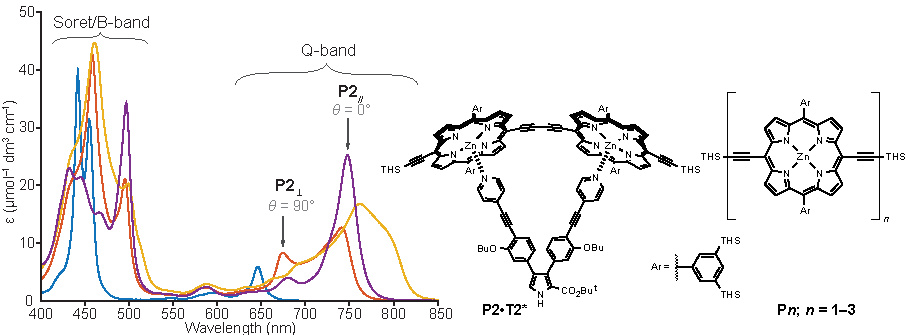
\includegraphics{figures/dimer/Figure-1.pdf} 
		\caption[]{Absorption spectra of linear oligomers: monomer \p1 (blue), dimer \p2 (red), trimer \p3 (yellow) and planar dimer complex \p2 $\bullet$ \textbf{T2} (purple). (Solvent: \ce{CH2Cl2}:THF:pyridine 10:10:1, except \p2$\bullet$\textbf{T2}: \dcm. THS = trihexylsilyl.)}
		\label{fig:dimer:f1}
	\end{figure}

	Previous semi-empirical and DFT calculations have predicted that the lowest energy conformation of \p2 is planar ($\theta = 0\degree$). These calculations gave a torsional energy barrier ($\Delta E$) of about \SIrange{3}{4}{\kjmol} (\autoref{table:dimer:t2}, \autoref{fig:dimer:f2}) between $\theta = 0\text{ and }90\degree$,\autocite{Lin1995,Stranger1996,Winters2007} which is in the range of $k_\text{B}T$ at room temperature (\SI{2.48}{\kjmol}), thus it is anticipated that all torsion angles are populated at room temperature. The barrier height was not significantly affected by the use of a range-separated DFT functional (CAM-B3LYP),\autocite{Yanai2004} an effective core potential, or a solvent model (\autoref{table:dimer:t2}). The torsion profile for the butadiyne linked dimer \p2 contrasts with that for the corresponding monoalkyne linked dimer\autocite{Lin1994}: in that case, coplanarity is disfavoured by the steric clash between porphyrin $\beta$ protons, and the DFT equilibrium torsion angle is about \SI{34}{\degree} (\autoref{fig:dimer:f2}). The $\Delta E$ between the equilibrium geometry and the perpendicular \SI{90}{\degree} conformer is around \SI{5}{\kilo\joule\per\mole}, greater than that in butadiyne linked \p2, and indicating increased conjugation across the linker. These computational results on \textbf{C\tsub2-}\p2 are in agreement with those found in several other studies, reviewed and contributed to by Rintoul \ltt{et al.},\autocite{Rintoul2013} who note that the computational equilibrium torsion angle (\textasciitilde{}\SI{35}{\degree}) is much greater than that expected from the narrow, redshifted absorption spectrum and than the angles observed in crystal structures (0--\SI{20}{\degree}).


	Computational work\autocite{Winters2007} (TD-DFT calculations, reproduced in this work, \autoref{fig:dimer:f4}) has shown that the visible electronic transitions of the butadiyne-linked porphyrin dimer exhibit a strong dependence on interporphyrin torsion angle $\theta$; as $\theta$ increases from 0 to 90\textdegree\ the Q-band transition is hypsochromically shifted. Torsion angle-dependence is also apparent in the B-band, albeit in the presence of several overlapping transitions.

	\begin{table}[ht!]
	\centering
		\caption[]{Molecular structures referred to in \autoref{table:dimer:t2} and in the present study}
		\label{table:dimer:t1}
	\begin{threeparttable}
	\begin{tabular}{ccccc}
	\multicolumn{5}{c}{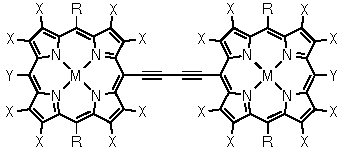
\includegraphics{figures/dimer/Table-1-Display.pdf}} \\
		\# & M & R & X & Y \\
		\midrule
		\cmpd{p2.a} & Ni & H & Et & H \\
		\cmpd{p2.b} & Zn & H & H & H \\
		\cmpd{p2.c} & Zn & Ph & H & \ce{C2H} \\
		\cmpd{p2.d} & Zn & Ph & H & \ce{C2SiMe3} \\
		\cmpd{p2.e}& Zn & H & H & \ce{C2H} \\
		\p2 & Zn & Ar\textsuperscript{\textdagger} & H & \ce{C2THS}\textsuperscript{\ddag} \\
		\bottomrule
	\end{tabular}
	\begin{tablenotes}
		\item \textdagger\ Ar $=$ 3,5-bis(trihexylsilyl) as defined in \autoref{fig:dimer:f1}. \item \ddag\ THS = trihexylsilyl.
	\end{tablenotes}
	\end{threeparttable}
	\end{table}

	\begin{table}[ht!]
	\centering
		\caption[]{Calculated barriers, $\Delta E$, to torsional rotation in butadiyne-linked porphyrin dimers}
		\label{table:dimer:t2}
	\begin{threeparttable}
	\begin{tabular}{cccc}
		Molecule & Method & $\Delta E$ (\si{\kjmol}) & Ref \\
		\midrule
		\cmpd{p2.a} & VWN and BP86 & $\sim\!63$ & \cite{Stranger1996} \\
		\cmpd{p2.b} & AM1 & $\sim\!4$ & \cite{Lin1995} \\
		\cmpd{p2.c} & B3LYP/6-31G* & 2.8 & \cite{Winters2007} \\
		\cmpd{p2.d} & B3LYP/6-31G*/LANL2DZ & 3.1\textsuperscript{\textdagger} & This work \\
		\cmpd{p2.d} & TPSSh/6-31G*/LANL2DZ & 3.7\textsuperscript{\textdagger}& This work \\
		\cmpd{p2.d} & CAM-B3LYP/6-31G* & 1.3\textsuperscript{\textdagger}& This work \\
		\cmpd{p2.d} & CAM-B3LYP/6-31G* \textsuperscript{\ddag} & 2.3\textsuperscript{\textdagger}& This work \\
		\cmpd{p2.d} & B3LYP/def2-SV(P) & 2.8\textsuperscript{\textdagger}& This work \\
		\cmpd{p2.e} & B3LYP/6-31G* & 2.6\textsuperscript{\textdagger}& This work \\
		\bottomrule
	\end{tabular}
	\begin{tablenotes}
		\item \textdagger\ No zero-point energy (ZPE)\nomenclature{ZPE}{Zero-point energy} correction applied. \item \ddag\ PCM\nomenclature{PCM}{Polarisable continuum model} THF solvent model.
	\end{tablenotes}
	\end{threeparttable}
	\end{table}



	\begin{figure}[ht!]
		\centering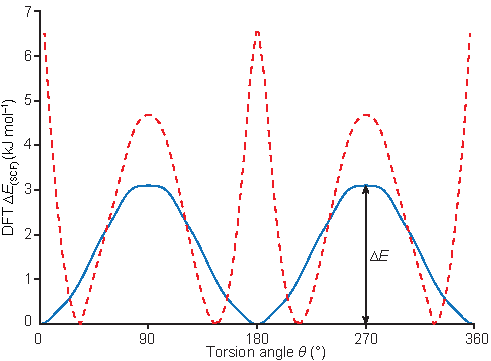
\includegraphics{figures/dimer/Figure-2b.pdf} 
		\caption[Calc. torsion profile for \p2]{Calculated (B3LYP/6-31G*/LANL2DZ) energy profile for butadiyne torsion in \p2, model \cmpd{p2.d} (blue). The red dashed line shows the torsion profile (B3LYP/6-31G*) for a monoalkyne linked analogue of \p2 (substitution pattern corresponding to model \cmpd{p2.b}). $\theta$ is the angle between the mean planes of each porphyrin, defined by the 24 non-hydrogen atoms in each macrocycle. The indicated $\Delta E$ is the torsional barrier for \p2 which is under discussion in this chapter.}
		\label{fig:dimer:f2}
	\end{figure}

	The torsion-dependence of the Q-band absorption wavelength has been exploited to selectively excite populations of molecules with different conformations. The wavelength of fluorescence emission is also dependent on the torsion angle. Analysis of fluorescence emission and excitation spectra shows that the \sing{1} state has a much higher torsion barrier (\SI{16}{\kjmol}) than the electronic ground state (\sing0).\autocite{Winters2007} Perpendicular conformers which are excited to \sing{1} tend to planarise prior to emission, unless solvent viscosity retards the rotation.\autocite{Winters2007,Kuimova2009,Kuimova2009b,Vyvsniauskas2015} The torsion angle has also been found to influence the two-photon absorption (2PA)\nomenclature{2PA}{Two-photon absorption} cross-section and the singlet oxygen (\ce{^{1}O_2}) yield. Planar conformers have stronger two-photon absorption,\autocite{Wilkinson2014} larger third-order optical non-linearities\autocite{Drobizhev2006} and higher charge-mobilities,\autocite{Grozema2007,Winters2007b} and they are more efficient oxygen sensitizers because intersystem crossing (\sing{1}$\rightarrow{}$\trip{1}) is faster than in twisted conformers.\autocite{Kuimova2009}

	The torsion angle can be constrained to enforce coplanarity by the preparation of supramolecular complexes, such as ladder complexes with a bidentate ligand (\ltt{e.g.} DABCO or 4,4\textprime-bipyridine),\autocite{Taylor1999} or simple 1:1 complexes between oligomers and designed templates, such as \textbf{T2} (\autoref{fig:dimer:f1}).\autocite{Winters2007,Winters2007b} Fixing the torsion angle results in the expected bathochromic shift and sharpening of the Q-band (\autoref{fig:dimer:f1}), as the conformation is restricted to a librational range of angles around $\theta \approx 0\degree$.

	Interestingly, Aida \ltt{et al.}\ prepared tetrameric cages from \textit{meso}-pyridyl substituted butadiyne-linked porphyrin dimers.\autocite{Tsuda2005} They found that the cage composed of dimer units with perpendicular porphyrins was favoured, due to the resulting cancellation of the pyridine dipole moments. This result showed that the torsion barrier in the butadiyne-linked dimer is low enough to be overcome by a dipole-based conformational preference.\autocite{Tsuda2005}

	The aim of this chapter is to experimentally determine the barrier to torsion in porphyrin dimer \p2 using VT UV-Vis-NIR spectroscopy and to understand how torsional rotation alters the electronic structure of this molecule. After presenting the VT UV-Vis-NIR results, we will discuss our theoretical analysis of the electronic excitations. With the help of this theoretical analysis, we will extract thermodynamic parameters using a van't Hoff analysis. We will use evidence from IR spectroscopy and bond-length alternation to discuss the resonance stabilisation of the planar conformer. Finally, we discuss our observation of helical frontier orbitals and natural transition orbitals in DFT calculations. 
	\FloatBarrier

	\section{Methods}

	\subsection{Synthesis and spectroscopy}

		Porphyrin compounds were prepared as described previously.\autocite{Grozema2007,Tait2015} Oligomers \textbf{P\textit{N}} with trihexylsilyl (THS) solubilising groups on the \textit{meso}-aryls were used throughout this study, since THS porphyrins exhibit excellent solubility and a low propensity towards aggregation. Room temperature UV-Vis-NIR spectra were recorded using a Perkin-Elmer Lambda 20 with a \SI{1}{\centi\metre} quartz cuvette. Variable temperature UV-Vis-NIR spectra were recorded using a Perkin-Elmer Lambda 1050 and an Oxford Instruments L\ce{N2} optical cryostat, with \SI{1}{\centi\metre} and \SI{1}{\milli\metre} Infrasil Quartz cuvettes (Starna). In all cases, freshly mixed \ce{CH2Cl2}:THF:pyridine (10:10:1) was used as the solvent mixture. \dcm and THF\nomenclature{THF}{Tetrahydrofuran} were dried over activated alumina before use. \dcm contained amylene (\SIrange{50}{150}{\ppm}) as a stabiliser; THF was unstabilised. Variable temperature UV-Vis-NIR experiments were performed across a wide concentration range (\SI{0.8}{\micro\Molar}, \SI{1.6}{\micro\Molar} and \SI{58.5}{\micro\Molar}) to confirm the absence of thermally-induced aggregation. Absorbances were not corrected for concentration change due to thermal contraction of the solvent, since the ratio of absorbances is not affected by concentration. Emission spectra were collected using an ISA Fluoromax-2 Fluorimeter. Infrared spectra were collected using a Bruker Tensor 27 FT-IR\nomenclature{FT}{Fourier transform} spectrometer in ATR mode with neat sample, with \SI{2}{\wn} resolution at \SI{293}{\kelvin}.

		%

	\subsection{Computational methods}

		All (TD-)DFT calculations were conducted using Gaussian09/D.01.\autocite{g09} The B3LYP density functional\autocite{Becke1993} was used in conjunction with the 6-31G* basis set,\autocite{Ditchfield1971,Hehre1972,Hariharan1973,Rassolov1998} with the LANL2DZ ECP\autocite{Hay1985a,Hay1985}\nomenclature{ECP}{Effective core potential} on Zn as indicated. For computational tractability, truncated model compounds were used. The potential-energy surface scan and TD-DFT calculations used a model of \p2 with phenyl substituents in place of the \textit{meso}-aryls, and trimethylsilyl protecting groups as the acetylene end-groups, and \symm{C}{1} symmetry, \cmpd{p2.d}. Further truncated models were used for the calculation of the vibronic fine structure of the Q-band transitions and vibrational frequencies: the \textit{meso}-aryls and the trimethylsilyl acetylene protecting groups were replaced by hydrogens, \cmpd{p2.e}. These calculations were then conducted in \symm{D}{2h} and \symm{D}{2d} symmetry for planar and perpendicular conformers respectively.

		The potential energy surface was calculated by varying the interporphyrin torsion angle in 2.5\textdegree{} increments and, while holding the torsion coordinate fixed, relaxing the remainder of the structure. The resulting $\Delta E_{SCF}$ is used for comparison: the zero-point vibrational contribution to the energy has been neglected unless indicated otherwise. Vibrational frequencies (calculated analytically, with the harmonic oscillator model) were scaled by a multiplicative factor of 0.96.

		Unless otherwise specified, orbital isosurfaces are depicted using the default threshold settings in the Chimera\autocite{pettersen2004ucsf} program. Namely, the thresholds are placed symmetrically about zero, at a value which encompasses 99\% of the voxels on either side of zero. 


\section{Results and discussion}
	\subsection{Experimental VT UV-Vis-NIR spectroscopy}

		Since the calculated torsion barrier $\Delta E$ is of the order of $k_{\text{B}} T$ at room temperature, we envisioned that VT UV-Vis-NIR spectroscopy would probe the equilibrium between twisted and planar conformers. Indeed, dramatic changes in the UV-Vis-NIR spectrum of \p2 (\SI{\sim{}59}{\micro\Molar}, \ce{CH2Cl2}:THF:pyridine 10:10:1) were observed upon cooling within the solvent liquid range (298–\SI{173}{\kelvin}, \autoref{fig:dimer:f3}). Below \SI{180}{\kelvin}, discontinuous changes in the spectra are observed, which we attribute to changes in bulk solvent properties at temperatures close to the glass transition temperature.\autocite{Bublitz1998}

		\begin{figure}[ht!]
			\centering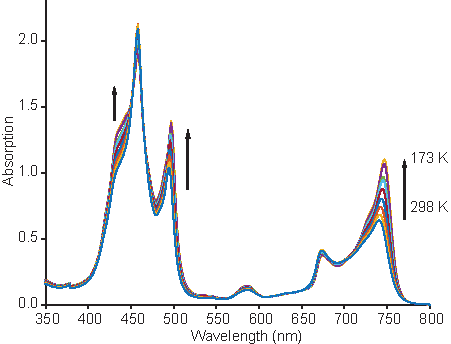
\includegraphics{figures/dimer/Figure-3.pdf} 
			\caption[]{Variable temperature (298–\SI{173}{\kelvin}) absorption spectra of porphyrin dimer \p2 in \ce{CH2Cl2}:THF:pyridine (10:10:1), concentration \ltt{ca.} \SI{59}{\micro\Molar}, path length \SI{1}{\milli\metre}.}
			\label{fig:dimer:f3}
		\end{figure}

		Previous work has shown that temperature-dependent changes in the absorption spectra of butadiyne-linked porphyrin oligomers can be caused by aggregation,\autocite{Karnbratt2012,Hutin2013} but as noted in the Methods, we were able to exclude the presence of aggregation by selection of appropriate solvent and solubilising side-chains. VT experiments performed on the porphyrin monomer \p1 in the same solvent mixture showed that, within the temperature range \SIrange{298}{163}{\kelvin}, there is no thermochromic shift of the Q-band absorption $\lambda$\textsubscript{max} (\autoref{fig:dimer:s1}).

		\begin{figure}[ht!]
			\centering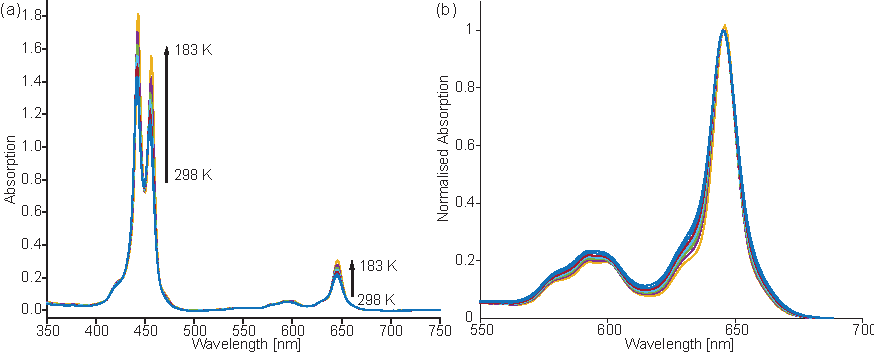
\includegraphics{figures/dimer/si-p1-vt-f1.pdf} 
			\caption[]{VT UV-­Vis spectra of monomer \p1 in \ce{CH2Cl2}:THF:pyridine 10:10:1, (a) full spectrum in temperature range
				298–77 K (b) expansion of Q-­band region in temperature range 298–\SI{163}{\kelvin}.}
			\label{fig:dimer:s1}
		\end{figure}

		When a solution of \p2 is cooled, its UV-Vis-NIR spectrum exhibits several changes (\autoref{fig:dimer:f3}): the red edge of the Q-band becomes more intense (\textasciitilde{}\SI{740}{\nano\metre}; planar conformations, $\theta \approx 0\degree$), at the expense of a slight decrease in intensity on the blue edge (\SI{675}{\nano\metre}; perpendicular conformations, $\theta \approx 90\degree$). We can be confident in our assignment of the absorbance at \SI{675}{\nano\metre} to perpendicular conformers thanks to measurements of the emission of twisted dimer conformers in viscous solution by Kuimova \ltt{et al.}\autocite{Kuimova2009b}, who found that highly viscous solvents inhibited excited state planarisation. The resulting emission, predominantly from twisted conformers, occurred bathochromically to the “shoulder” on the high-energy side of the Q-band absorption. 

		The absorption at \SI{570}{\nano\metre}, assigned with the help of TD-DFT to near-planar conformers (see later), increases intensity on cooling. In the Soret/B-band, a sharpening and intensification of the absorption on the red edge is observed (\textasciitilde{}\SI{490}{\nano\metre}). This band can thus also be assigned to near-planar conformers. Before discussing the van't Hoff analysis of the VT UV-Vis-NIR of \p2, we will further develop our understanding of the absorption spectra using TD-DFT\@.
		\FloatBarrier
	\subsection{Calculated electronic transitions as a function of torsion angle}

		We computed the electronic excitations for different torsion angles using TD-DFT (B3LYP/6-31G*/LANL2DZ) (\autoref{fig:dimer:f4}). The results agree with earlier published work.\autocite{Winters2007} The transition dipole moments for the lowest energy part of the Q-band are polarised along the butadiyne (long, \textit{x}) axis, as observed experimentally.\autocite{Anderson1994a,Drobizhev2005} Analysis of the angle dependence of the Q-band excitation energy reveals a relationship to $\cos \theta$: \ltt{i.e.}, the projection of the porphyrin planes (\autoref{fig:dimer:f5}), as given by equation (\ref{eqn:qband-cos}):

		\begin{figure}[ht!]
			\centering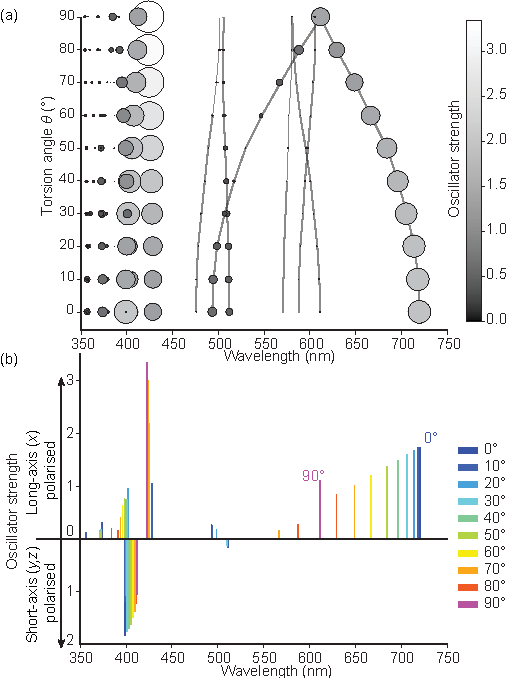
\includegraphics{figures/dimer/Figure-4.pdf} 
			\caption[]{Calculated (TD-B3LYP/6-31G*/LANL2DZ) vertical excitation energies in the UV-Vis-NIR region for different torsion angles in a model \p2 (\cmpd{p2.d}). (a) Calculated wavelength \ltt{vs.} torsion angle. Faint grey lines (only shown for the Q-bands) connect corresponding states, comprising a Walsh diagram; circle size is proportional to oscillator strength, as is the circle shading. (b) Calculated wavelength \ltt{vs.} oscillator strength. Transitions with oscillator strength \textless 0.1 are not included. Bars above the x-axis correspond to transitions polarised along the long molecular axis ($x$, butadiyne axis) of the molecules. Bars below the $x$-axis correspond to transitions polarised along either the $y$ or $z$ (short) molecular axes.}
			\label{fig:dimer:f4}
		\end{figure}

		\begin{figure}[ht!]
			\centering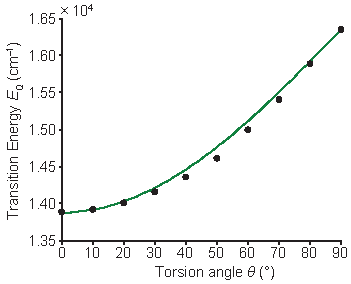
\includegraphics{figures/dimer/Figure-5.pdf} 
			\caption[]{Comparison of TD-DFT calculated \sing0$\rightarrow{}$\sing1 vertical excitation energy (blue) \ltt{vs.} a predictive model based on the projection of the porphyrin planes (green) (\eref{eqn:qband-cos}).}
			\label{fig:dimer:f5}
		\end{figure}

		\begin{equation}\label{eqn:qband-cos}
		E_Q \approx E_\bot - (E_\bot - E_\parallel)\cdot \cos \theta
		\end{equation}

		\noindent{}where $E_Q$ is the Q-band absorption energy for a conformer with inter-porphyrin torsion angle $\theta$. $E_\parallel$ and $E_\bot$ are the limiting energies for planar (low energy) and perpendicular (high energy) conformers, respectively. This function readily relates absorption energy to the overlap of the porphyrin \pii-systems along the butadiyne and shows that $E_Q$ is most sensitive to $\theta$ when $\theta \approx 90\degree$.

		The calculated oscillator strength of the lowest energy transition is surprisingly high for the 90\textdegree{} conformer (\autoref{fig:dimer:f4}b), contrasting its gradual decrease with increasing $\theta$ between 0–80\textdegree{}. This result does not appear to be a simple computational artefact: the increase of oscillator strength is gradual from 85--90\textdegree{} (\autoref{fig:dimer:s2}). Close examination of the TD-DFT results reveals that, on twisting from 0--90\textdegree{}, the second-lowest energy \textit{x}-axis (long axis) polarised transition is progressively redshifted until it becomes degenerate with the lowest energy transition (\autoref{fig:dimer:f4}a). This analysis further reveals that the weak absorption centred at \textasciitilde{}\SI{580}{\nano\metre} in the experimental spectrum (\autoref{fig:dimer:f1}) arises predominantly from planar conformers, and contains components polarised along both the long (\textit{x}) and short (\textit{y}) molecular axes. A detailed discussion of TD-DFT results and orbital/state correlations as a function of torsion angle has been published previously by Winters \ltt{et al.}, and our computational results are in complete agreement with theirs.\autocite{Winters2007}

		\begin{figure}[ht!]
			\centering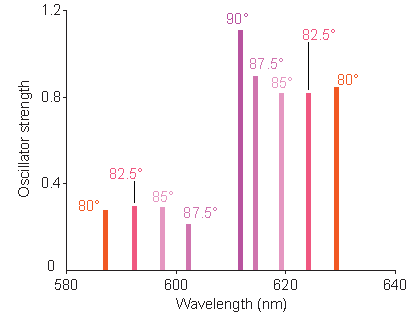
\includegraphics{figures/dimer/si-small-angles-f2.pdf} 
			\caption[]{TD-DFT (B3LYP/6-31G*/LANL2DZ) calculated excitation energies and oscillator strengths for \p2 (model \cmpd{p2.d}) as a function of inter-­porphyrin torsion angle}
			\label{fig:dimer:s2}
		\end{figure}

		The high oscillator strength of the Q band of the perpendicular conformer ($\theta = 90\degree$) provides a partial explanation for the peak observed in the absorption spectrum at \SI{675}{\nano\metre} (\figplural \ref{fig:dimer:f1} and \ref{fig:dimer:f3}). However, a further contribution appears likely because the peak at \SI{675}{\nano\metre} persists at low temperature, with similar relative intensity to the planar conformer as at room temperature. Even at \SI{78}{\kelvin}, at which temperature occupation of the perpendicular state should be thermally inhibited, there is a discrete absorption at \textasciitilde{}\SI{675}{\nano\metre} (\autoref{fig:dimer:f6}). Room temperature emission spectra of \p2 and \p2$\bullet$\textbf{T2} (\figplural \ref{fig:dimer:s7comb}a and \ref{fig:dimer:s7comb}b) show a similar shoulder on the red edge of the main emission band. Therefore we assign this shoulder to a vibronic contribution of the planar conformer, with the support of computational results described in the next section.

		\begin{figure}[ht!]
			\centering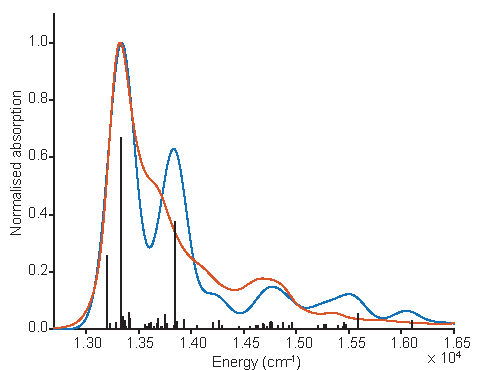
\includegraphics{figures/dimer/Figure-6.pdf} 
			\caption[]{(red) Absorption spectrum of Q-band region (600–\SI{800}{\nano\metre}) of \p2 in frozen solution (\ce{CH2Cl2}:THF:pyridine 10:10:1) at \SI{78}{\kelvin}; (blue) calculated (B3LYP/6‑31G* Franck-Condon/Herzberg-Teller approximation) vibronic structure of Q-band absorption for planar \p2, model \cmpd{p2.e}; (sticks) vibronic transitions; transitions with low relative intensity are not plotted. The $\langle0|0\rangle$ transition in the computational result was shifted in energy to match the low-energy peak in the experimental spectrum (red).}
			\label{fig:dimer:f6}
		\end{figure}

		\begin{figure}[ht!]
			\centering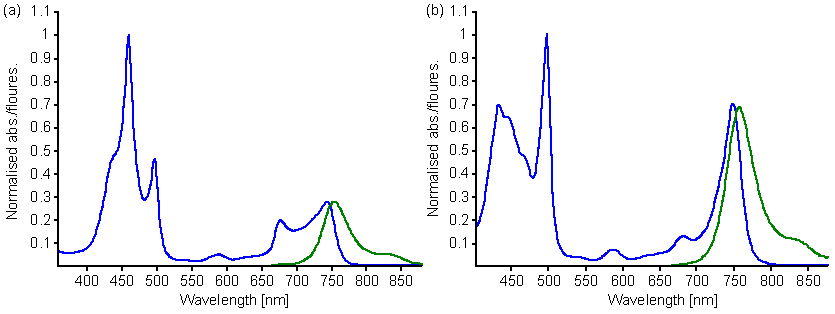
\includegraphics{figures/dimer/si-p2fl-comb.pdf} 
			\caption[]{Absorption (blue) and fluorescence (green) of (a) \p2 (\ce{CHCl3} + 1\% pyridine), $\lambda_{ex} = 450$ nm and (b) \p2$\bullet$\textbf{T2} (\ce{CHCl3}), $\lambda_{ex} = 450$ nm, $\lambda_{max}(\log_{10} \epsilon)$: 749 (5.297), 682 (4.574), 588 (4.324), 498 (5.452), 434 (5.295).}
			\label{fig:dimer:s7comb}
		\end{figure}

		\FloatBarrier
	\subsection{Vibronic contribution to the Q-band electronic transition}

		We used the Franck-Condon (FC)\nomenclature{FC}{Franck-Condon} and Herzberg-Teller (HT)\nomenclature{HT}{Herzberg-Teller} approximations as implemented in Gaussian09/D.01 to calculate the vibronic absorption spectrum for the \sing0$\rightarrow{}$\sing1 transition in planar \p2.\autocite{Santoro2008,Barone2009} The calculation was restricted to excitations originating from the vibrational ground state of \sing0, thus treating the vibronic spectrum as temperature independent. This calculation gave a predicted spectrum which is in remarkably close agreement to the experimental spectrum of \p2 recorded at \SI{78}{\kelvin} (\autoref{fig:dimer:f6}). At this temperature the near-planar conformers of \p2 are expected to be dominantly populated. The major vibronic bands arise from intra-porphyrin collective stretching modes, and do not appear to involve nuclear displacements on the butadiyne link (see \autoref{fig:dimer:s3}). The vibronic band which we calculate at \SI{\sim 390}{\wn} from the $\langle0|0\rangle$ transition has also been experimentally characterised by Camargo \ltt{et al.}\ in \p1, at \SI{380}{\wn}.\autocite{Camargo2015} We used the computational vibronic spectrum to firmly assign the absorption at \SI{675}{\nano\metre} in (planar) \p2$\bullet$\textbf{T2} (\autoref{fig:dimer:f1}) to a vibronic contribution. Similarly, the anomalously increased intensity at the blue edge of the Q-band (\textasciitilde{}\SI{675}{\nano\metre}) in the experimental spectra of \p2 at room temperature (\autoref{fig:dimer:f1}) is partially attributed to this vibronic contribution, in addition to the relatively high oscillator strength of the overlapping perpendicular absorption. The significant overlap between the absorption of the twisted conformer and that of a vibronic band of the planar conformer rationalises previous results where wavelength-selective excitation of the twisted conformer appeared to result, additionally, in excitation of the planar conformer.\autocite{Winters2007,Wilkinson2014} 

		\begin{figure}[ht!]
			\centering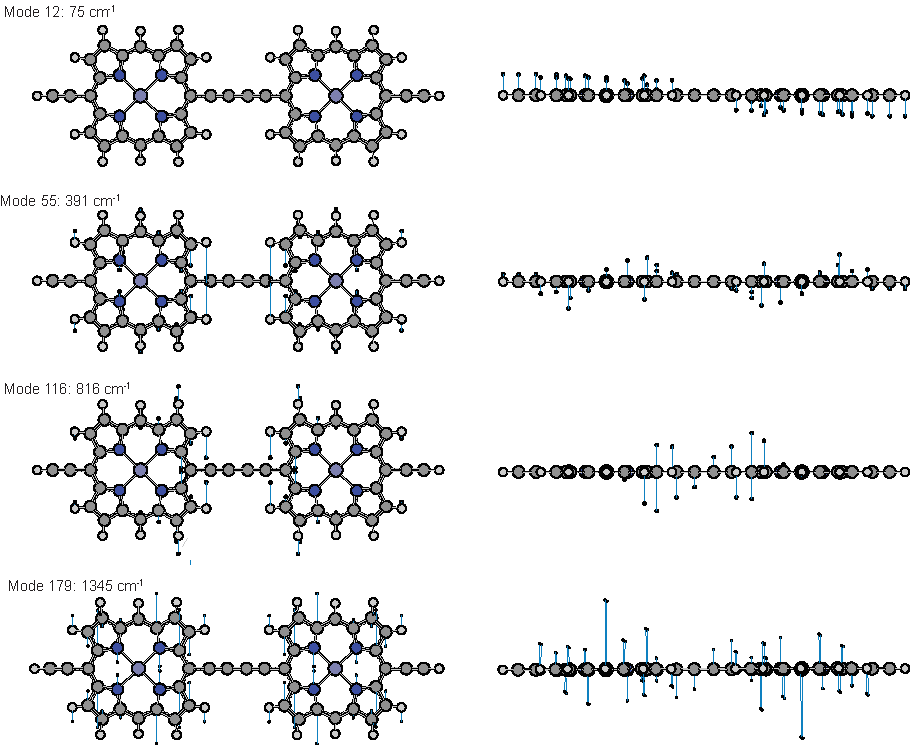
\includegraphics{figures/dimer/si-vibrations-s3.pdf} 
			\caption[]{Normal modes of \sing1 state of \p2 (model \cmpd{p2.e}) associated with major vibronic bands.}
			\label{fig:dimer:s3}
		\end{figure}
		\FloatBarrier
	\subsection{van't Hoff analysis of experimental VT UV-Vis-NIR data}

		The experimental VT UV-Vis-NIR data were subject to a van't Hoff analysis of the equilibrium constant for a simple two-state model comprising near-planar and near-perpendicular conformers, \p2$_\parallel$ ($\theta \approx 0\degree$) and \p2$_\bot$ ($\theta \approx 90\degree$) with concentrations proportional to the absorbances at 750 and \SI{675}{\nano\metre}, respectively, weighted by the TD-DFT oscillator strengths for the 0\textdegree{} and 90\textdegree{} transitions.\footnote[3]{We also used the van't Hoff equation without weighting the absorbances at 750 and \SI{675}{\nano\metre} to the calculated oscillator strengths.  This approach does not change the resulting value of \delh{} ($\SI{5.27 \pm 0.03}{\kjmol}$), but it gives a higher value of \dels{} ($\SI{14.42 \pm 0.14}{\jkmol}$); thus, $\Delta{}G_{\text{298 K}}$ becomes $\SI{0.98 \pm 0.05}{\kjmol}$ } The vibronic contribution of the planar conformer to the absorption at \SI{675}{\nano\metre} (mostly perpendicular conformer) was subtracted. The relative magnitude of this vibronic contribution was assumed to be temperature-invariant and was calculated from the ratio of peak heights in the spectrum of \p2 at \SI{78}{\kelvin}. 

		The equilibrium constant at each temperature was thus calculated according to equation (\ref{eqn:eqconstant}):

		\begin{equation}\label{eqn:eqconstant}
		K = \frac{f_\parallel}{f_\bot} \cdot \frac{A_\bot}{A_\parallel} = \frac{f_\parallel}{f_\bot} \cdot \frac{A_{675} - A_{750} \cdot x_{vibr}}{A_{750}}
		\end{equation}

		where $K$ is the equilibrium constant for:
		\begin{center}
			\ce{\textbf{P2}_$\parallel$ <=>[{$K$}][] \textbf{P2}_$\bot$}
		\end{center}

		$A_\parallel$ and $A_\bot$ are the absorbances for planar and perpendicular conformers, respectively. $f_\parallel$ and $f_\bot$ are the TD-DFT oscillator strengths for planar and perpendicular conformers, respectively ($\frac{f_\parallel}{f_\bot} = 1.574$). $x_{vibr}$ is the ratio of the intensities of the planar $\langle0|0\rangle$ absorption and its vibronic contribution (at \SI{\sim 1350}{\wn} separation) in the experimental \SI{78}{\kelvin} spectrum of \p2 ($x_{vibr} = 0.186$). The ratio of TD-DFT oscillator strengths (1.574) is consistent with the ratio of estimated experimental extinction coefficients for the planar and perpendicular conformers. The experimental ratio of extinction coefficients for planar and perpendicular conformers ($\frac{\epsilon_{\parallel}}{\epsilon_{\bot}}$) was estimated by comparing the absorption coefficients of free \p2 (in the presence of pyridine) and complexed \p2$\bullet$\textbf{T2} at \SI{750}{\nano\metre} (planar, $\epsilon_{\parallel}$) and \SI{675}{\nano\metre} (perpendicular, $\epsilon_{\bot}$), after subtraction of the vibronic contribution at \SI{675}{\nano\metre} in free \p2. The vibronic contribution in liquid solution at room temperature is given by the following equation, assuming that in \p2$\bullet$\textbf{T2}, there is no perpendicular \p2 (\ltt{i.e.}, all absorption at \SI{675}{\nano\metre} arises from the vibronic contribution).

		\begin{equation}
			x_{vibr}= \frac{\epsilon_{\SI{675}{\nano\metre}, \textbf{T2}}}{\epsilon_{\SI{750}{\nano\metre}, \textbf{T2}}} = 0.171
		\end{equation}

		Thus $\epsilon_\bot$ can be estimated by subtracting this vibronic contribution:

		\begin{equation}
			\epsilon_{\bot, py} = x_{vibr} \times \epsilon_{\SI{675}{\nano\metre}, py} = \SI{60960}{\per\Molar\per\centi\metre} 
		\end{equation}

		Where $\epsilon_{py}$ corresponds to spectra recorded in the presence of pyridine, and $\epsilon_{\textbf{T2}}$ to the complex \p2$\bullet$\textbf{T2}. Next we calculate $\Delta \epsilon_\parallel$. $\Delta \epsilon_\bot$ was found in the previous step (\SI{60960}{\per\Molar\per\centi\metre}) assuming all \p2 has been planarised.

		\begin{equation}
			\Delta \epsilon_\parallel = \epsilon_{\SI{750}{\nano\metre}, \textbf{T2}} = \epsilon_{\SI{750}{\nano\metre}, py} = \SI{103990}{\per\Molar\per\centi\metre} 
		\end{equation}

		Thus:

		\begin{equation}
		\frac{\Delta \epsilon_\parallel}{\Delta \epsilon_\bot} = \frac{\num{103990}}{\num{60960}} = 1.7059
		\end{equation}


		Within the temperature range 298–\SI{198}{\kelvin}, the van't Hoff plot (\autoref{fig:dimer:f7}) of the extracted equilibrium constants shows an excellent straight-line fit, and is concentration independent across the range measured (\SIrange{0.8}{59}{\micro\Molar}), thus excluding the presence of aggregation. Thermodynamic parameters were extracted: $\delh = \SI{5.27 \pm 0.03}{\kilo\joule\per\mole}$ (in reasonable agreement with most computational estimates, \autoref{table:dimer:t2}), $\dels = \SI{10.69 \pm 0.14}{\joule\per\kelvin\per\mole}$. The large value of \dels demonstrates an important temperature dependence for the rotational barrier: $\Delta G_{\SI{298}{\kelvin}} = \SI{2.08 \pm 0.05}{\kilo\joule\per\mole}$;  $\Delta G_{\SI{180}{\kelvin}} = \SI{3.35 \pm 0.04}{\kilo\joule\per\mole}$ -- in other words, the barrier rises as the temperature falls.

		\begin{figure}[ht!]
			\centering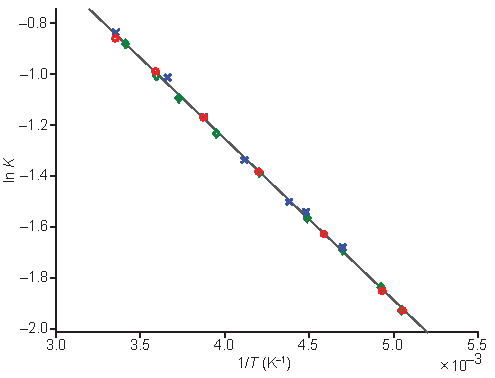
\includegraphics{figures/dimer/Figure-7.pdf} 
			\caption[]{van't Hoff plot and fit line for VT experiments at three different concentrations: \SI{0.8}{\micro\Molar} (blue crosses), \SI{1.6}{\micro\Molar} (green diamonds), \SI{58.5}{\micro\Molar} (red circles). $R^{2} = 0.999$.}
			\label{fig:dimer:f7}
		\end{figure}

		There are few previous reports of the determination of both \delh and \dels for a torsional equilibrium. Our thermodynamic parameters for \p2 are similar to those reported for \textit{trans}-\textit{skew} isomerism in 1,1-dihalo-3-fluoro-buta-1,3-dienes from solution-phase IR spectroscopy (halo = Br: $\delh = \SI{3.53}{\kilo\joule\per\mole}$, $\dels = \SI{3.5}{\joule\per\kelvin\per\mole}$; halo = Cl: $\delh = \SI{2.95}{\kilo\joule\per\mole}$, $\dels = \SI{2.3}{\joule\per\kelvin\per\mole}$).\autocite{Hartman1968} \dels for oxalyl chloride (\textit{trans}-\textit{gauche} isomerism) has been calculated from the experimental vibrational modes (excluding the torsion mode) as \SI{\sim{}13}{\jkmol},\autocite{Durig1992} and from gas-phase electron diffraction as \SI{10}{\jkmol}.\autocite{Hagen1973} We attribute our positive value of \dels to changes in the frequencies of large-amplitude (low frequency) motions between the planar and twisted states, including the pertinent torsion mode and butadiyne bending modes.

		The potential energy surface from DFT calculations (\autoref{fig:dimer:f2}) was scaled based on the experimentally determined thermodynamic parameters (\delh and \dels), and the Boltzmann equation (\autoref{eqn:dimer:boltz}) was used to determine the temperature dependence of the mole fraction of each conformer (\autoref{fig:dimer:f8}). Inclusion of the entropic factor in this manner permits a more accurate simulation of temperature-dependent populations than simply using a temperature-independent barrier height, which would overestimate conformational heterogeneity at low temperature, and underestimate it at high temperatures.

		\begin{equation}\label{eqn:dimer:boltz}
			%\frac{N_j}{N_i} = \frac{g_j}{g_i} \me^{-\frac{E_j - E_i}{k_\text{B}T}}
			p_i = \frac{\me^{-\frac{E_i}{k_\text{B}T}}}{\sum_{j=1}^M \me^{-\frac{E_j}{k_\text{B}T}}}
		\end{equation}
		\noindent{}where $p_i$ is the population of the $i$\nth state, $k_\text{B}T$ is the Boltzmann constant, and $E_i$ is the relative energy of the $i$\nth state. 

		\begin{figure}[ht!]
			\centering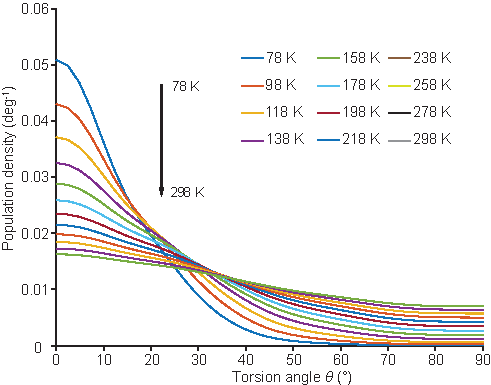
\includegraphics{figures/dimer/Figure-8.pdf} 
			\caption[]{Temperature dependence of the population density for different torsion angles, based on the experimentally determined \delh and \dels.}
			\label{fig:dimer:f8}
		\end{figure}

		The stated error in our thermodynamic parameters is the error in the fit of the experimental data to the van't Hoff equation, and must be taken in the context of the approximation of the two-state model. Our analysis presents a lower bound for the torsion barrier height, because the model evaluates the barrier between near-planar and near-perpendicular conformers. Spectral overlap between angles in a small range (estimated 0–20\textdegree{}) around 0\textdegree{} and 90\textdegree{} means that the absorptions at \SI{750}{\nano\metre} and \SI{675}{\nano\metre} capture some contributions from nearby angles.
		\FloatBarrier
	\subsection{Evidence for enhanced conjugation in the planar conformer from C$\equiv$C bond length and vibrational frequencies}

		The torsion barrier for \p2, $\delh = \SI{5.27}{\kilo\joule\per\mole}$, can be compared to that for other alkyne- and butadiyne-linked molecules. The experimental torsion barrier of tolane (Ph–C$\equiv$C–Ph) is \SI{2.42}{\kilo\joule\per\mole},\autocite{Okuyama1984} compared to the near-barrierless (\SI{0.05}{\kilo\joule\per\mole}) torsion of di\-methyl\-acetylene (Me–$\equiv$–Me).\autocite{Olson1971} Calculations have indicated that the barrier for diphenyldiacetylene (DPDA, Ph–C$\equiv$C–C$\equiv$C–Ph) is around \SI{1.1}{\kilo\joule\per\mole} (PBE0/6-31+G*//6-31G* and B3LYP/6-31+G**).\autocite{Thulstrup2011,Sebree2012} 

		1,4-Bis(phenylethynyl)benzene (Ph–C$\equiv$C–C$_6$H$_4$–C$\equiv$C–Ph) has an experimental barrier of \SI{2.75}{\kilo\joule\per\mole}, similar to that for tolane, but DFT (B3LYP/6-31G**) dramatically overestimates the barrier at \SI{8.75}{\kjmol}.\autocite{Greaves2006}

		To ensure comparability of computational results, we have calculated the torsion barrier of tolane and DPDA\nomenclature{DPDA}{Diphenyldiacetylene} at the B3LYP/6-31G* level of theory, by performing constrained geometry optimisations of planar and perpendicular conformers. At this level of theory, the barrier for DPDA is \SI{1.1}{\kjmol}, while that for tolane is \SI{3.8}{\kjmol} (calculated in this work, and in agreement with previously published data\autocite{Wierzbicka2015}).

		One might expect the torsion barrier to increase with the ability of the \pii-system at each end of the butadiyne to stabilise radical or anionic/cationic character, as a consequence of contributions from cumulenic resonance forms in the ground state (\autoref{fig:dimer:f9}a). Such contributions should be reflected in a decrease in the bond length alternation (BLA) in the butadiyne link (\autoref{fig:dimer:f9}b). This hypothesis is supported by our computational studies: the BLA in planar \p2 (\cmpd{p2.d}, \SI{0.151}{\angstrom}) is smaller than that in DPDA (\SI{0.158}{\angstrom}) as shown in \autoref{table:dimer:t3}. We used the range-separated CAM-B3LYP\autocite{Yanai2004} functional in this part of the study: CAM-B3LYP gave BLAs in closer agreement to crystal structures than B3LYP\@. The more accurate estimation of BLA in polyynes when using DFT functionals with increased exact exchange (BHHLYP and CAM-B3LYP \ltt{vs.} B3LYP) has been reported.\autocite{Peach2007}

		\begin{figure}[ht!]
			\centering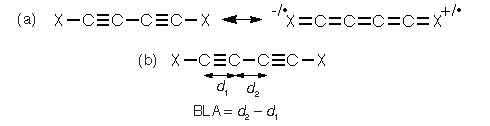
\includegraphics[width=0.7\textwidth]{figures/dimer/Figure-9.pdf} 
			\caption[]{(a) A butadiyne-linked conjugated compound can be considered a combination of both alternant and cumulenic forms. The alternant form is dominant. (b) The relative contributions of these resonance structures can be estimated from the bond length alternation.}
			\label{fig:dimer:f9}
		\end{figure}

		The calculated BLA for perpendicular \p2 (\SI{0.163}{\angstrom}) is higher than for planar \p2 (\SI{0.151}{\angstrom}), and is even higher than both conformations of DPDA (\SI{0.158}{\angstrom}). This change in the nature of bonding between perpendicular and planar \p2 further supports the hypothesis that resonance delocalisation via a cumulenic canonical form is important in the planar conformer. The resonance stabilisation in DPDA is demonstrably lower – the calculated BLA is the same in perpendicular and planar conformers.



		\begin{table}[ht!]
				\setlength\dashlinedash{0.4pt}
				\setlength\dashlinegap{1.5pt}
				\setlength\arrayrulewidth{0.3pt}
			\centering
			\caption[]{Calculated and crystallographic bond length alternation (BLA) in \cmpd{p2.d} and DPDA}
			\label{table:dimer:t3}
		%\begin{threeparttable}
		\begin{tabular}{cccc}
			Molecule & Method & Conformer & BLA(\angstrom{}) \\
			\midrule
			\multirow{3}{*}{\cmpd{p2.d}} & \multirow{2}{*}{CAM-B3LYP/6-31G*} & $\theta = 90 \degree$ & 0.163 \\
			 &  & $\theta = 0 \degree$ & 0.151 \\
			 & crystal structure \autocite{Taylor1998,Berlicka2005,Chen2006} & $\theta = 0 \degree$ & $0.165 \pm 0.007$ \\
			 \hdashline
			\multirow{3}{*}{DPDA} & \multirow{2}{*}{CAM-B3LYP/6-31G*} &  $\theta = 90 \degree$ & 0.158 \\
			 &  & $\theta = 0 \degree$ & 0.158 \\
			 & crystal structure\autocite{Coates1997a,Glock2013,Gdaniec2003,Surette1994,Fronczek1995,Shi2006a} & $\theta = 0 \degree$ & $0.178 \pm 0.011$ \\
			\bottomrule
		\end{tabular}
		%\begin{tablenotes}
		%\end{tablenotes}
		%\end{threeparttable}
		\end{table}

		We have also compared BLA in crystal structures of \p2 \ltt{vs.}\ DPDA\@. We used ConQuest\autocite{Bruno2002} to search the Cambridge Crystallographic Structure Database.\autocite{Allen2002} After rejection of one DPDA structure with a high R-value (9.2\%),\autocite{Thomas2009} we did indeed find that the mean BLA in butadiyne-linked porphyrin dimers (average of 3 structures) is less than that in unsubstituted DPDA (average of 6 structures, \autoref{table:dimer:t3}). However, the difference has low statistical significance ($p = 0.067$, Welch’s \textit{t}-statistic) and the sample sizes are too small to permit an unequivocal conclusion. Thus, we consider the evidence for resonance stabilisation from BLA analyses of crystal structures provisional: as more accurate crystallographic data become available, it may be possible to perform a more definitive analysis. 

		A contribution from cumulenic resonance forms should also be apparent in the frequency of the butadiyne $\nu_{\text{C}\equiv{}\text{C}}$ asymmetric stretch, observable by IR spectroscopy (\SIrange{2100}{2200}{\wn}). We,\autocite{Movsisyan2014} and others,\autocite{Yildizhan2011} have previously used IR spectroscopy to explore cumulenic character in electronic excited states of polyynes. Increasing cumulenic character results in a lower frequency vibration. Experimentally, we see a \SI{13}{\wn} difference for the $\nu_{\text{C}\equiv{}\text{C}}$ in experimental ATR\nomenclature{ATR}{Attenuated total reflectance} FT-IR spectra of DPDA (\SI{2147}{\wn}) compared with \p2 (\SI{2134}{\wn}) (\autoref{table:dimer:t4}). These results are in reasonable agreement with calculation (\autoref{table:dimer:t4}). It is clear from the IR and crystallographic BLA\nomenclature{BLA}{Bond-length alternation} that the contribution of cumulenic resonance structures to the bonding in \p2 is very small, as reflected in the low barrier to torsional rotation, but that it is greater than in DPDA\@.

		\begin{table}[ht!]
			\centering
			\caption[]{Experimental and calculated acetylene stretch frequencies $\nu_{\text{C}\equiv{}\text{C}}$}
			\label{table:dimer:t4}
		\begin{threeparttable}
		\begin{tabular}{ccc}
			Molecule & Method & $\nu_{\text{C}\equiv{}\text{C}}$ \wnum \\
			\midrule
			\multirow{2}{*}{\cmpd{p2.e} (\sing0)} & Expt. & 2134  \\
			 & B3LYP/6-31G* \textsuperscript{\textdagger} & 2132 (2120)\textsuperscript{\textdaggerdbl}  \\
			 \hdashline
			 \cmpd{p2.e} (\sing1) & TD-B3LYP/6-31G* \textsuperscript{\textdagger} &  2078 (2109)\textsuperscript{\textdaggerdbl} \\
			 \hdashline	
			 \multirow{2}{*}{DPDA} & Expt. &  2147 \\
			 & B3LYP/6-31G* \textsuperscript{\textdagger} & 2156 \\
			 \bottomrule
		\end{tabular}
		\begin{tablenotes}
			\item \textdagger Planar conformer, frequencies scaled by a multiplicative factor 0.96.
			\item \textdaggerdbl Terminal alkyne stretch
		\end{tablenotes}
		\end{threeparttable}
		\end{table}


		The calculated vibrational frequencies of \p2 in its \sing1 excited state show far more cumulenic character with a lower $\nu_{\text{C}\equiv{}\text{C}}$ (\SI{2078}{\wn}, \autoref{table:dimer:t4}), correlating with the increased torsion barrier (16 \kjmol) in \sing1.\autocite{Winters2007} This result suggests that time-resolved IR spectroscopy could be used to probe the extent and dynamics of conjugation in the excited states of butadiyne-linked oligomers. We have previously used this technique to show cumulenic character in the first singlet and triplet excited states of a hexayne chain.\autocite{Movsisyan2014}
		\FloatBarrier
	\subsection{Helical molecular orbitals in twisted conformers}

		To offer further insight into the nature of the Q-band (\sing0$\rightarrow{}$\sing1) excitations, we have calculated the natural transition orbitals (NTOs)\autocite{Martin2003} for both planar and perpendicular \p2 (\autoref{fig:dimer:f10}). The NTOs provide an intuitive picture of the natural orbital origin of the hole and electron involved in a transition. Multiple electron/hole NTO pairs may be used to describe a single transition: the relative contribution of each electron/hole pair representation to the TD-DFT transition density is denoted by an eigenvalue ($\lambda$). The NTO pair describing the \sing0$\rightarrow{}$\sing1 (Q-band) transition in planar \p2, ($\theta = 0\degree$, \autoref{fig:dimer:f10}a) shows, as expected, the absence of charge transfer character in the excitation. Both hole and electron are delocalised over both porphyrin units. 

		\begin{figure}[ht!]
			\centering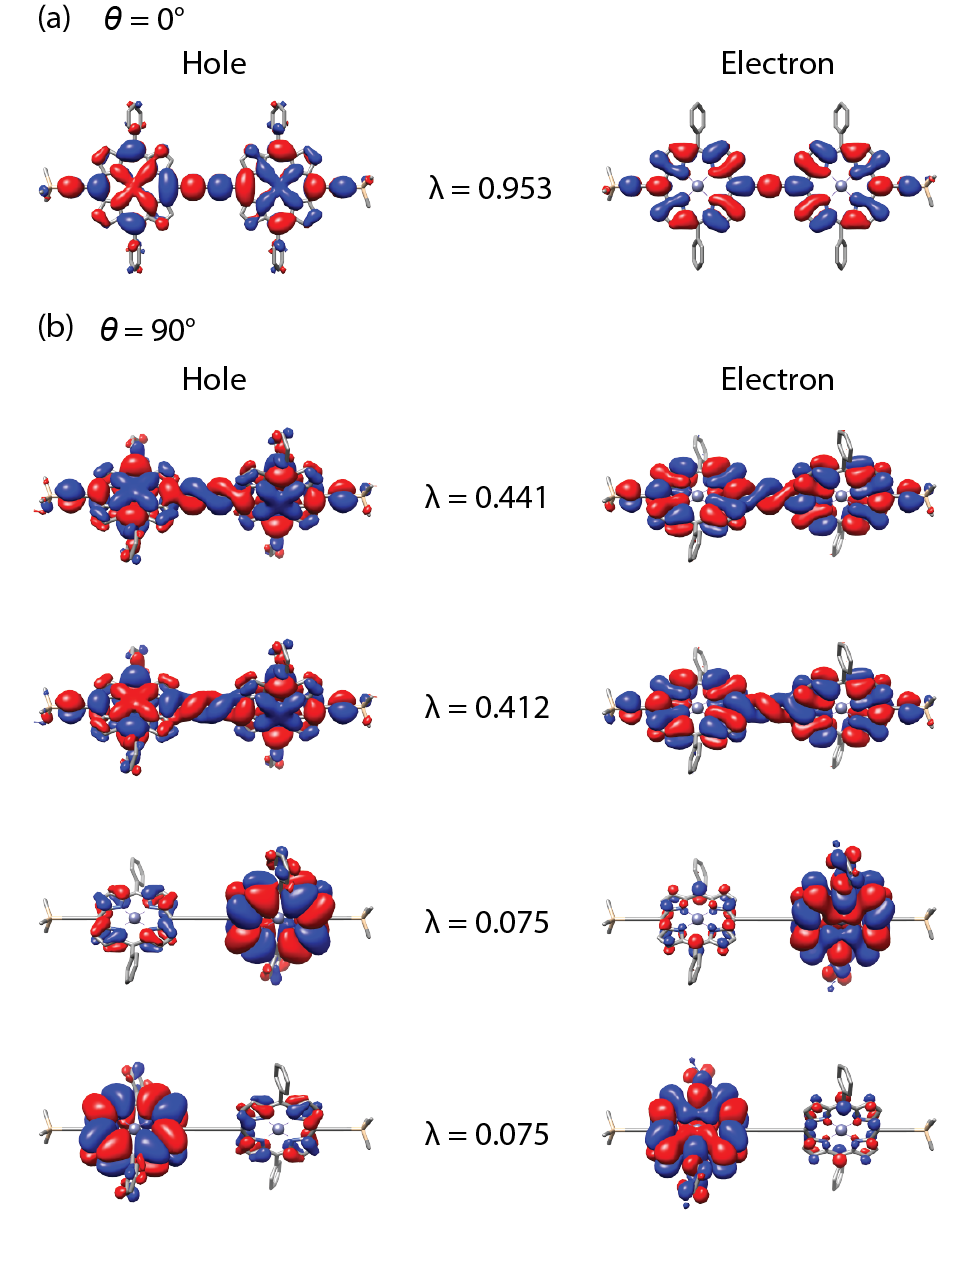
\includegraphics{figures/dimer/Figure-10.png} 
			\caption[]{Natural transition orbitals (NTOs) calculated at the B3LYP/6-31G* level of theory for (a) planar and (b) perpendicular conformers of \cmpd{p2.d}. The eigenvalue associated with each NTO hole/electron pair is shown as $\lambda$. The default isovalues are depicted (for $\theta = \SI{0}{\degree}$, $\sim$0.01\~a.u.; for $\theta = \SI{90}{\degree}$, $\sim$0.008\~a.u. and $\sim$0.005\~a.u. for $\lambda \approx 0.4$ and $\lambda \approx 0.08$, respectively.)}
			\label{fig:dimer:f10}
		\end{figure}

		Interestingly, the first two NTOs\nomenclature{NTO}{Natural transition orbital} of perpendicular \p2 ($\theta = 90\degree$, \autoref{fig:dimer:f10}b) show that this excitation can be largely described (\textasciitilde{}85\%) with both hole and electron delocalised over both porphyrin units through apparent helical orbital character on the butadiyne link, arising from admixture of the perpendicular $\pi_x$ and $\pi_y$ butadiyne orbitals. The NTOs for \p2 are similar to the HOMO\nomenclature{HOMO}{Highest occupied MO} and LUMO\nomenclature{LUMO}{Lowest unoccupied MO} for the planar and perpendicular conformers (\autoref{fig:dimer:s5}), reflecting the predominantly HOMO--LUMO nature of the \sing0$\rightarrow{}$\sing1 transition. Helical butadiyne orbitals are also observed for the HOMO and LUMO of twisted conformers of \p2, with increasing admixture of $\pi_x$ and $\pi_y$ orbitals upon twisting (\autoref{fig:dimer:s5}). Similar effects have been observed in calculations on the much simpler DPDA.\autocite{Thulstrup2011} The reported effects of endgroup torsion on the DFT frontier orbital energies in DPDA\autocite{Thulstrup2011} are similar to those reported in our previous work for \p2.\autocite{Winters2007} Helical orbitals have previously been calculated by DFT for some cumulene/polyyne molecules.\autocite{Hendon2013,Liu2013} However, we are reluctant to attach much significance to the helicity in the NTOs and frontier orbitals of \p2: the first two NTOs are pseudo-enantiomeric and near degenerate ($\lambda = 0.441$ and $\lambda = 0.412$), and their structures differ only in the phase of localised orbitals on the left hand porphyrin, and in the handedness of the helical portion of the MO\@. Degeneracy is broken due to the lack of symmetry in this model: the \textit{meso}-aryl groups and terminal trimethylsilylacetylenes result in \symm{C}{1} symmetry. A similar calculation performed with a truncated model (\symm{D}{2d} symmetry) gave a degenerate pair of orthogonal NTOs, with no orbital helicity (\autoref{fig:dimer:s4}). Similarly, the frontier orbitals in this symmetric model show no helical orbital character (\autoref{fig:dimer:f11}).



		\begin{figure}[ht!]
			\centering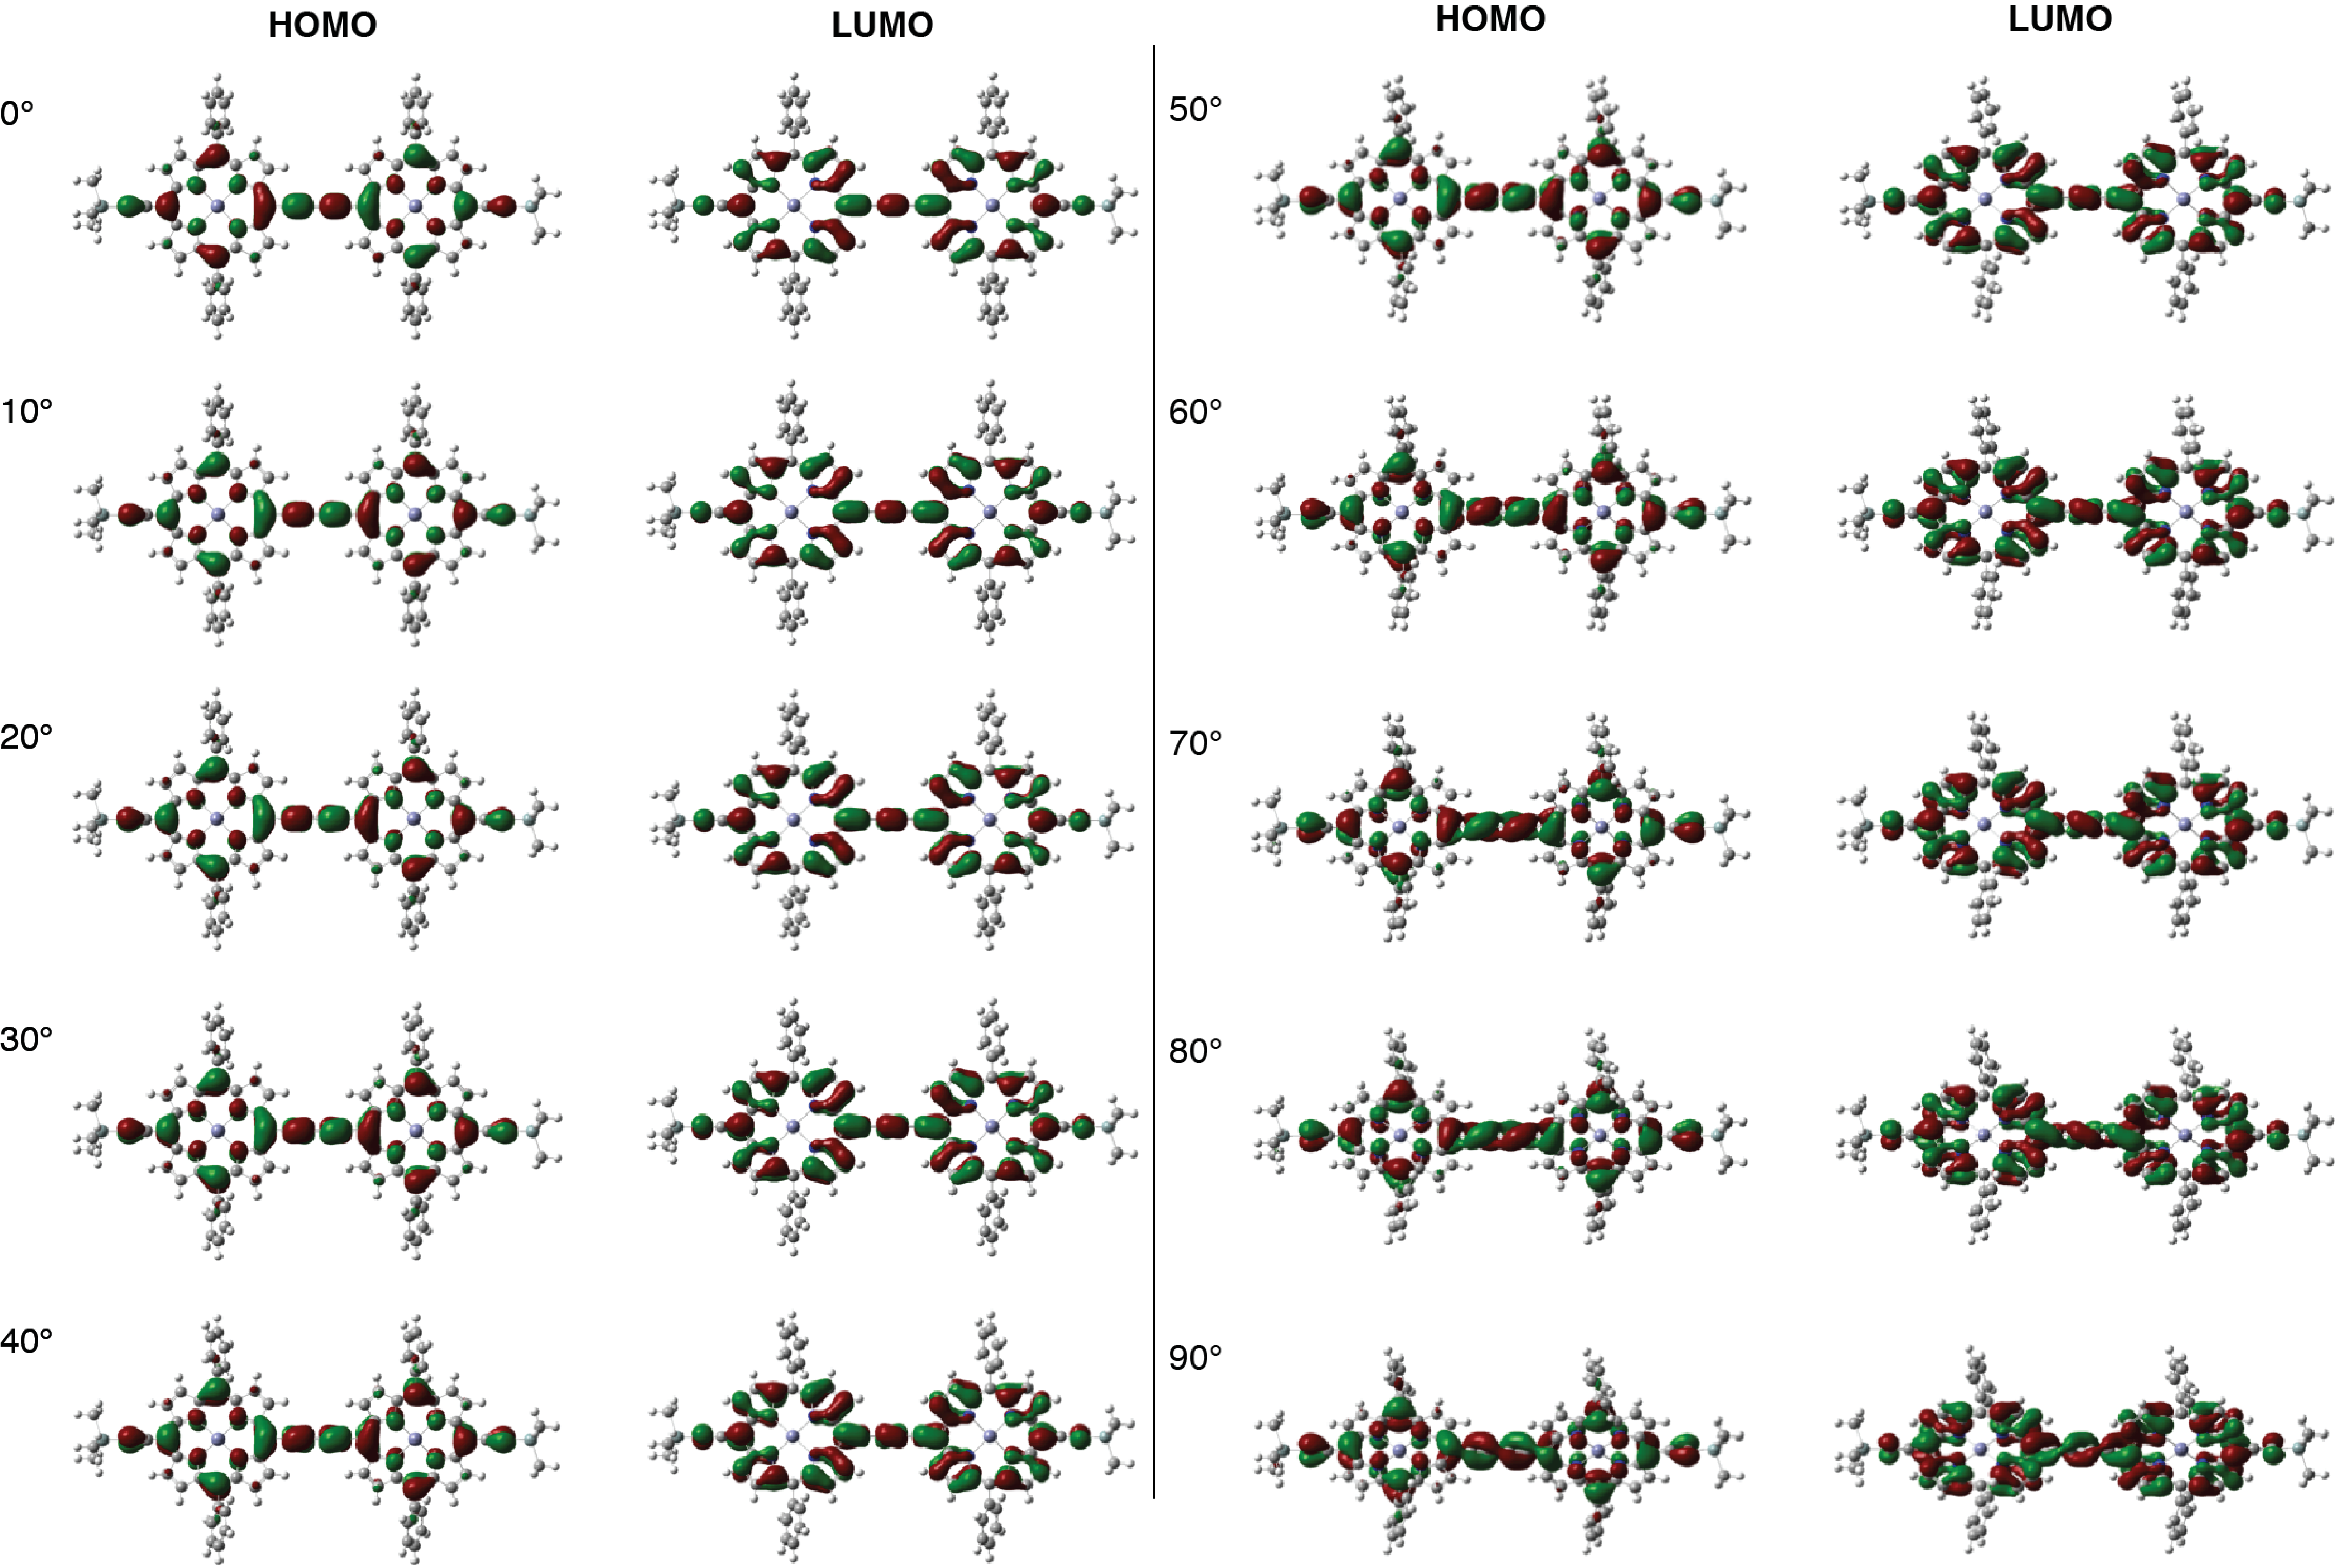
\includegraphics[width=\textwidth]{figures/dimer/homo-lumo.png} 
			\caption[]{DFT (B3LYP/6-31G*/LANL2DZ) HOMO and LUMO for \p2 (model \cmpd{p2.d}) as a function of interporphyrin torsion angle, 0–90\textdegree. The default isovalues are used, which are typically 0.08 to 0.15\~a.u.}
			\label{fig:dimer:s5}
		\end{figure}

		% \begin{figure}
		% 	\centering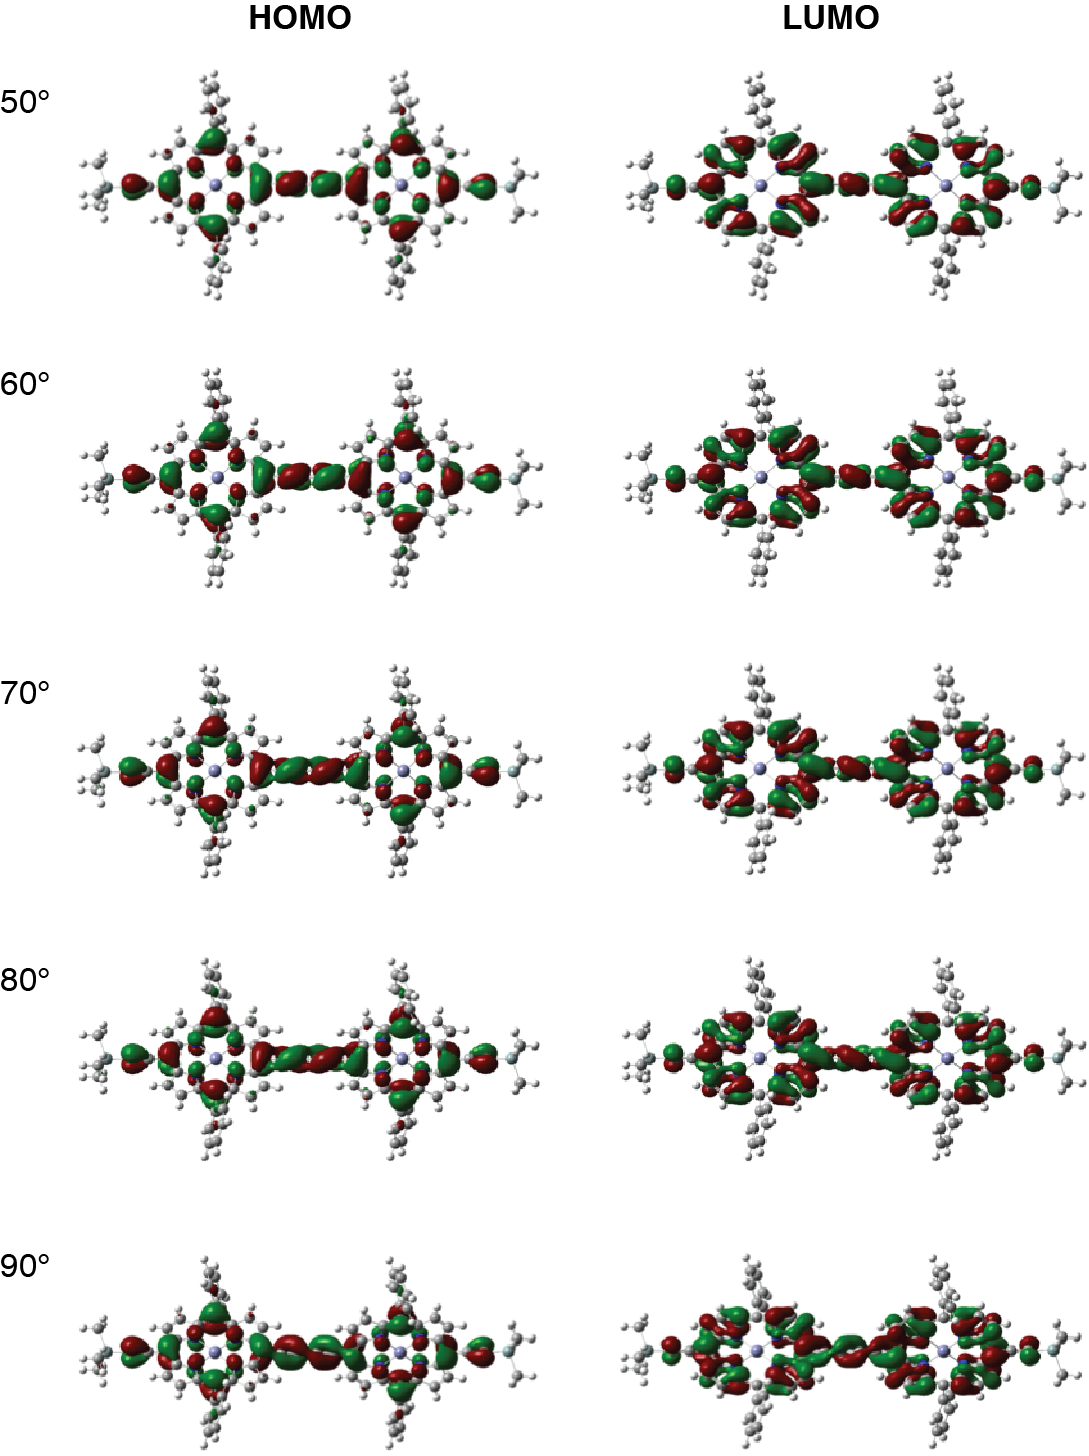
\includegraphics[width=0.5\textwidth]{figures/dimer/si-s6.png} 
		% 	\caption[]{DFT (B3LYP/6-31G*/LANL2DZ) HOMO and LUMO for \p2 (model \cmpd{p2.d}) as a function of interporphyrin torsion angle, 50–90\textdegree}
		% 	\label{fig:dimer:s6}
		% \end{figure}

		\begin{figure}[ht!]
			\centering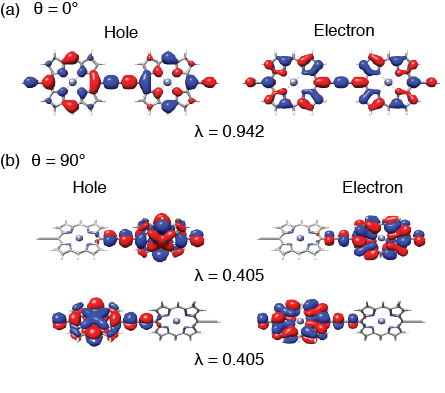
\includegraphics{figures/dimer/si-s4.png} 
			\caption[]{Natural transition orbitals (NTOs) for \sing0~$\rightarrow$~\sing1 transition calculated (TD-B3LYP/6-­31G*) for model \cmpd{p2.e}. The eigenvalue associated with each NTO hole/electron pair is shown as $\lambda$. The default isovalues are used, which for all parts of the figure are $\sim$0.15\~a.u.}
			\label{fig:dimer:s4}
		\end{figure}

		\begin{figure}[ht!]
			\centering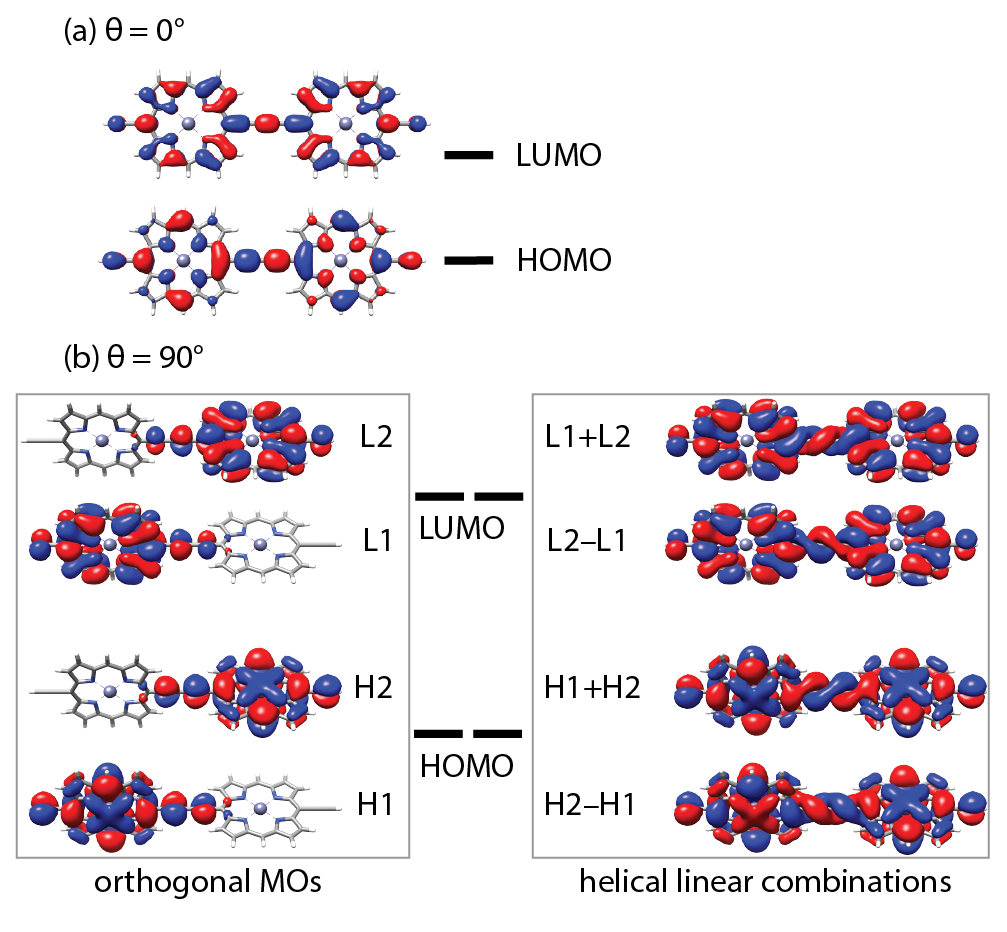
\includegraphics{figures/dimer/Figure-11.png} 
			\caption[]{(a) Degenerate HOMO and LUMO of planar (\symm{D}{2h}) \p2 (model \cmpd{p2.e}); (b) degenerate HOMO and LUMO of perpendicular (\symm{D}{2d}) \cmpd{p2.e} (left) and linear combinations of the same orbitals (right), showing helical character. The default isovalues are used, which for all parts of the figure are $\sim$0.15\~a.u.}
			\label{fig:dimer:f11}
		\end{figure}


		The equivalence of helical and localised MO\nomenclature{MO}{Molecular orbital} representations is demonstrated by taking linear combinations of the (originally orthogonal) degenerate HOMO and LUMO of a twisted conformer (\symm{D}{2d} symmetry, B3LYP/6-31G*, \autoref{fig:dimer:f11}), giving non-orthogonal but degenerate helical orbitals. For example, in the $\theta = 90\degree$ conformation of \cmpd{p2.e}, there are two degenerate HOMOs, H1 and H2, each localised on one porphyrin unit; the sum and difference of these orbitals (H1 + H2 and H2 – H1) are helical, enantiomeric and degenerate. In the present study, we have found that helical orbitals occur where there is a deviation from \symm{D}{2d} symmetry (and hence frontier orbital degeneracy) in twisted conformers, either due to non-symmetric molecular structures (disordered sidegroups) or due to geometry relaxation to a minimum with a value of $\theta$ close to, but not exactly 90\textdegree{}. 
		\FloatBarrier

\section{Conclusions}

	The barrier to torsion about the butadiyne link in a porphyrin dimer has been determined experimentally by VT UV-Vis-NIR absorption spectroscopy. The planarisation of a twisted dimer was analysed with a van't Hoff treatment to yield the following thermodynamic parameters for planarisation: $\delh = \SI{5.27 \pm 0.03}{\kjmol}$ and $\dels = \SI{10.69 \pm 0.14}{\jkmol}$. 

	(TD-)DFT calculations were used on model systems to explore the suitability of computational methods for the study of these chromophores. Gratifyingly, an affordable DFT functional/basis set combination (B3LYP/6-31G*) provided a barrier height in reasonable agreement with experiment, and TD-DFT results permitted clear characterisation of the dimer Q-band, in agreement with previous work.\autocite{Winters2007} In particular, the use of TD-DFT\nomenclature{TD-DFT}{Time-dependent DFT} to assign vibronic structure in the Q-band absorption was essential for the deconvolution of overlapping spectral features for the van't Hoff analysis and afforded theoretical insight into previous wavelength-selective excitation studies.

	The torsion barrier in \p2 is higher than that calculated for 1,4-diphenylbutadiyne, suggesting that the increase in the size of the conjugated endcapping \pii-system increases the barrier height, owing to increased resonance stabilisation. Examination of the experimental $\nu_{\text{C}\equiv{}\text{C}}$ IR stretch and calculated BLAs offer some support to this rationale.



